\scanpage{154}
% 154.01 Top, cancelled tensor and four terms with overlapping braces
\[
\deleted{E_1\otimes E_2}\quad
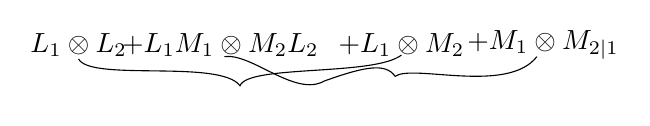
\begin{tikzpicture}[baseline=(a.base)]
\node[inner sep=1pt] (a) at (0,0) {$L_1\otimes L_2$};
\node[inner sep=1pt] (b) at (1.8,0) {$+\deleted{L_1}M_1\otimes\deleted{\unsure{M_2}}L_2$};
\node[inner sep=1pt] (c) at (4.1,0) {$+L_1\otimes M_2$};
\node[inner sep=1pt] (d) at (5.9,0) {$+M_1\otimes M_{\unsure{2|1}}$};
\draw (0,-.18) .. controls (.15,-.47) and (1.8,-.18) .. (2.05,-.52) .. controls (2.15,-.25) and (3.75,-.4) .. (4.1,-.13);
\draw (1.85,-.15) .. controls (2.2,-.1) and (2.75,-.67) .. (3.12,-.46) .. controls (3.65,-.27) and (3.9,-.23) .. (4.02,-.4) .. controls (4.24,-.24) and (5.45,-.63) .. (5.82,-.15);
\end{tikzpicture}
\]

% 154.02 Upper left, diagram in three levels
\diagram{\begin{tikzcd}[ampersand replacement=\&,column sep=small,row sep=small]
E_1\otimes_{0}E_2\arrow[rr,"F_{11}^{!}"]\arrow[dr,"\pi"]\arrow[dd]\arrow[ddrrr,bend right=30,dash]
\&{}\&E_1\otimes E_2\arrow[rr]\&{}\&E_1\otimes^{0}E_2\\
{}\&L_1\otimes L_{\unsure{2|12}}\arrow[ur,"\alpha_1\otimes\alpha_2"']\&{}\&\text{\deleted{\unsure{confusi|conveni|connu}\,\unsure{ment|avec|}}}\&{}\\
E_1\otimes\unsure{E_2|\Omega}\arrow[rrr,dash,"\psi_1\otimes\psi_2"']\&{}\&{}\&M_1\otimes M_2\arrow[uur]\&{}
\end{tikzcd}}

% 154.03 Upper right, two factors
\[(E_1\otimes M_2)\times(M_1\otimes E_2)\]

% 154.04 Above table, three objects
\diagram{\begin{tikzcd}[ampersand replacement=\&]
L_1\otimes L_2\arrow[r,dash]\&\otimes\arrow[r,dash]\&\otimes
\end{tikzcd}}

% 154.05 Immediately above table
\[\unsure{\mathbb Z|\xi}\]

% 154.06 Centre, four by four table
\diagram{$\begin{array}{c|cccc}
 &L_1\deleted{\unsure{\otimes}}\otimes L_2 & L_1\otimes M_2 & M_1\otimes L_2 & M_1\otimes M_2\\ \hline
L_1\otimes L_2 &\chi&\mathrm{id}_{L_1}\otimes\tau_2&\tau_1\otimes\mathrm{id}_{L_2}&?\ (T_1\otimes T_2\,?)\\
L_1\otimes M_2 &0&0&0&\underline{?}\ \cdot\tau_1\otimes\mathrm{id}_{M_2}\\
M_1\otimes L_2 &0&0&0&\underline{?}\ \deleted{\unsure{\tau_2}}\mathrm{id}_{M_1}\otimes\tau_2\\
M_1\otimes M_{1} &0&0&0&\chi
\end{array}$}

% 154.07 Below table, three lines and right-hand addition
On \unsure{trouve} que les 2 \deleted{\unsure{compositions}}\inserted{\unsure{homomorphismes de}} \unsure{carré|coïnc.|connues}\inserted{ sur $E_{\unsure{11|12}}$} sont compatibles, et laissent une \unsure{indétermination|indéterminée}, qui est un hom de $M_1\otimes M_2$ en $L_1\otimes L_2$.

% 154.08 Lower centre, two columns of working
\[
\begin{aligned}
-\qquad E_1\otimes E_2 &\qquad E_1\otimes E_2\\
\pi'_1=\alpha_1\pi_1\ \big/\ \unsure{\omega'_1|\varpi'_1}=\varpi_1\psi_1&\qquad \pi'_1+\varpi\\
\pi'_2=\alpha_2\pi_2\qquad\varpi'_2=\omega_2\psi_2&
\end{aligned}
\]

% 154.09 Foot, three lines
C'est normal, car pour l'instant on n'a \unsure{rien|écrit} \uline{que} le fait qu'on veut une \unsure{iso|paire|loi} d'extensions - \deleted{\unsure{et}} celles-ci sont \unsure{triviales|toutes}, on a l'embarras du choix !
% archive sheet number: 153
